% Created by tikzDevice version 0.12.6 on 2024-02-25 11:57:50
% !TEX encoding = UTF-8 Unicode
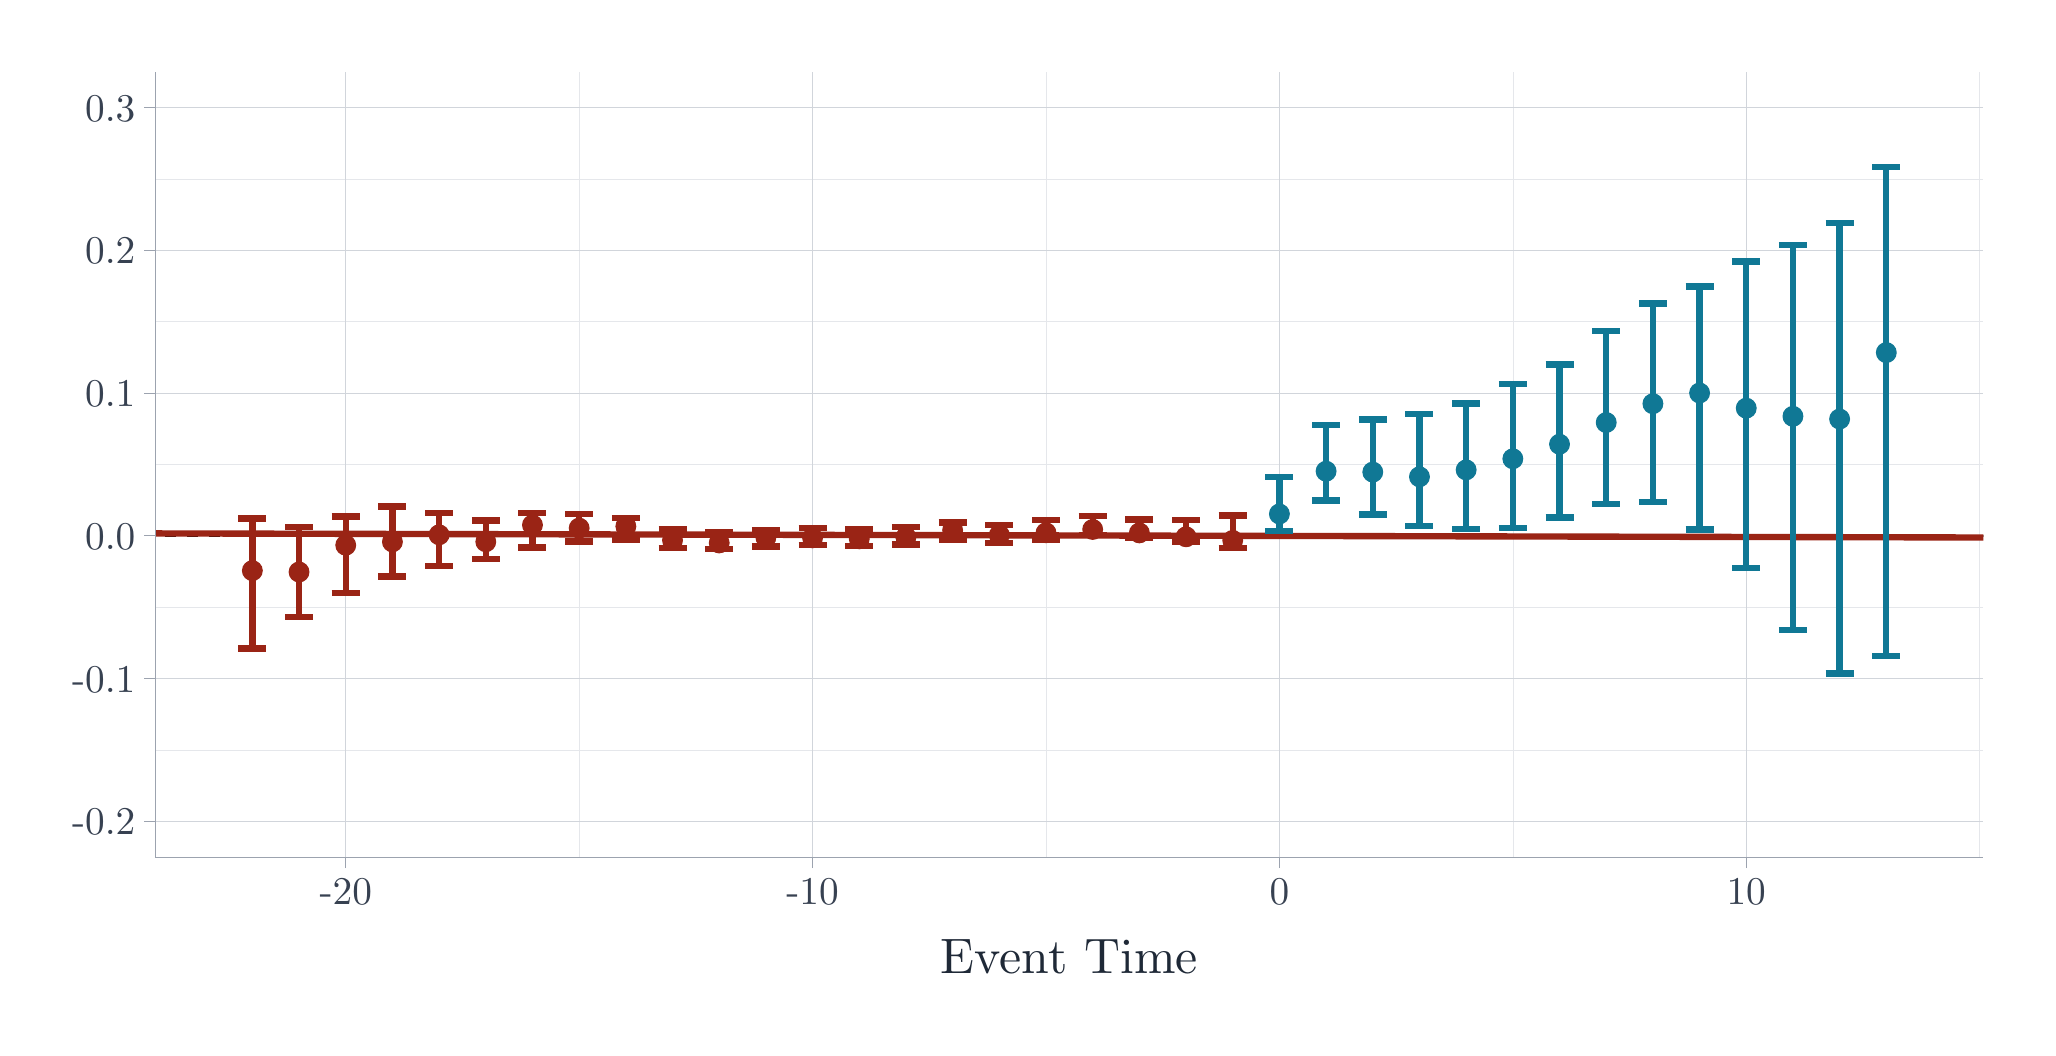
\begin{tikzpicture}[x=1pt,y=1pt]
\definecolor{fillColor}{RGB}{255,255,255}
\path[use as bounding box,fill=fillColor] (0,0) rectangle (722.70,361.35);
\begin{scope}
\path[clip] (  0.00,  0.00) rectangle (722.70,361.35);
\definecolor{drawColor}{RGB}{255,255,255}

\path[draw=drawColor,line width= 0.8pt,line join=round,line cap=round,fill=fillColor] (  0.00,  0.00) rectangle (722.70,361.35);
\end{scope}
\begin{scope}
\path[clip] ( 46.10, 61.65) rectangle (706.70,345.35);
\definecolor{drawColor}{RGB}{255,255,255}
\definecolor{fillColor}{RGB}{255,255,255}

\path[draw=drawColor,line width= 0.8pt,line join=round,line cap=round,fill=fillColor] ( 46.10, 61.65) rectangle (706.70,345.35);
\definecolor{drawColor}{RGB}{229,231,235}

\path[draw=drawColor,line width= 0.2pt,line join=round] ( 46.10,100.34) --
	(706.70,100.34);

\path[draw=drawColor,line width= 0.2pt,line join=round] ( 46.10,151.92) --
	(706.70,151.92);

\path[draw=drawColor,line width= 0.2pt,line join=round] ( 46.10,203.50) --
	(706.70,203.50);

\path[draw=drawColor,line width= 0.2pt,line join=round] ( 46.10,255.08) --
	(706.70,255.08);

\path[draw=drawColor,line width= 0.2pt,line join=round] ( 46.10,306.66) --
	(706.70,306.66);

\path[draw=drawColor,line width= 0.2pt,line join=round] (199.28, 61.65) --
	(199.28,345.35);

\path[draw=drawColor,line width= 0.2pt,line join=round] (367.97, 61.65) --
	(367.97,345.35);

\path[draw=drawColor,line width= 0.2pt,line join=round] (536.66, 61.65) --
	(536.66,345.35);

\path[draw=drawColor,line width= 0.2pt,line join=round] (705.35, 61.65) --
	(705.35,345.35);
\definecolor{drawColor}{RGB}{209,213,219}

\path[draw=drawColor,line width= 0.4pt,line join=round] ( 46.10, 74.55) --
	(706.70, 74.55);

\path[draw=drawColor,line width= 0.4pt,line join=round] ( 46.10,126.13) --
	(706.70,126.13);

\path[draw=drawColor,line width= 0.4pt,line join=round] ( 46.10,177.71) --
	(706.70,177.71);

\path[draw=drawColor,line width= 0.4pt,line join=round] ( 46.10,229.29) --
	(706.70,229.29);

\path[draw=drawColor,line width= 0.4pt,line join=round] ( 46.10,280.87) --
	(706.70,280.87);

\path[draw=drawColor,line width= 0.4pt,line join=round] ( 46.10,332.45) --
	(706.70,332.45);

\path[draw=drawColor,line width= 0.4pt,line join=round] (114.93, 61.65) --
	(114.93,345.35);

\path[draw=drawColor,line width= 0.4pt,line join=round] (283.62, 61.65) --
	(283.62,345.35);

\path[draw=drawColor,line width= 0.4pt,line join=round] (452.31, 61.65) --
	(452.31,345.35);

\path[draw=drawColor,line width= 0.4pt,line join=round] (621.00, 61.65) --
	(621.00,345.35);
\definecolor{drawColor}{RGB}{0,0,0}

\path[draw=drawColor,line width= 0.9pt,dash pattern=on 4pt off 4pt ,line join=round] (-614.49,177.71) -- (1367.30,177.71);
\definecolor{drawColor}{RGB}{154,36,21}

\path[draw=drawColor,line width= 2.3pt,line join=round] (-614.49,180.07) -- (1367.30,175.65);
\definecolor{fillColor}{RGB}{154,36,21}

\path[draw=drawColor,line width= 0.4pt,line join=round,line cap=round,fill=fillColor] ( 81.19,165.14) circle (  3.57);

\path[draw=drawColor,line width= 0.4pt,line join=round,line cap=round,fill=fillColor] ( 98.06,164.66) circle (  3.57);

\path[draw=drawColor,line width= 0.4pt,line join=round,line cap=round,fill=fillColor] (114.93,174.34) circle (  3.57);

\path[draw=drawColor,line width= 0.4pt,line join=round,line cap=round,fill=fillColor] (131.80,175.54) circle (  3.57);

\path[draw=drawColor,line width= 0.4pt,line join=round,line cap=round,fill=fillColor] (148.67,178.09) circle (  3.57);

\path[draw=drawColor,line width= 0.4pt,line join=round,line cap=round,fill=fillColor] (165.54,175.58) circle (  3.57);

\path[draw=drawColor,line width= 0.4pt,line join=round,line cap=round,fill=fillColor] (182.41,181.64) circle (  3.57);

\path[draw=drawColor,line width= 0.4pt,line join=round,line cap=round,fill=fillColor] (199.28,180.51) circle (  3.57);

\path[draw=drawColor,line width= 0.4pt,line join=round,line cap=round,fill=fillColor] (216.15,181.16) circle (  3.57);

\path[draw=drawColor,line width= 0.4pt,line join=round,line cap=round,fill=fillColor] (233.01,176.11) circle (  3.57);

\path[draw=drawColor,line width= 0.4pt,line join=round,line cap=round,fill=fillColor] (249.88,175.15) circle (  3.57);

\path[draw=drawColor,line width= 0.4pt,line join=round,line cap=round,fill=fillColor] (266.75,177.12) circle (  3.57);

\path[draw=drawColor,line width= 0.4pt,line join=round,line cap=round,fill=fillColor] (283.62,177.00) circle (  3.57);

\path[draw=drawColor,line width= 0.4pt,line join=round,line cap=round,fill=fillColor] (300.49,176.64) circle (  3.57);

\path[draw=drawColor,line width= 0.4pt,line join=round,line cap=round,fill=fillColor] (317.36,177.27) circle (  3.57);

\path[draw=drawColor,line width= 0.4pt,line join=round,line cap=round,fill=fillColor] (334.23,179.76) circle (  3.57);

\path[draw=drawColor,line width= 0.4pt,line join=round,line cap=round,fill=fillColor] (351.10,178.06) circle (  3.57);

\path[draw=drawColor,line width= 0.4pt,line join=round,line cap=round,fill=fillColor] (367.97,178.83) circle (  3.57);

\path[draw=drawColor,line width= 0.4pt,line join=round,line cap=round,fill=fillColor] (384.84,180.03) circle (  3.57);

\path[draw=drawColor,line width= 0.4pt,line join=round,line cap=round,fill=fillColor] (401.71,178.78) circle (  3.57);

\path[draw=drawColor,line width= 0.4pt,line join=round,line cap=round,fill=fillColor] (418.58,177.37) circle (  3.57);

\path[draw=drawColor,line width= 0.4pt,line join=round,line cap=round,fill=fillColor] (435.44,176.07) circle (  3.57);
\definecolor{drawColor}{RGB}{16,120,149}
\definecolor{fillColor}{RGB}{16,120,149}

\path[draw=drawColor,line width= 0.4pt,line join=round,line cap=round,fill=fillColor] (452.31,185.63) circle (  3.57);

\path[draw=drawColor,line width= 0.4pt,line join=round,line cap=round,fill=fillColor] (469.18,201.08) circle (  3.57);

\path[draw=drawColor,line width= 0.4pt,line join=round,line cap=round,fill=fillColor] (486.05,200.76) circle (  3.57);

\path[draw=drawColor,line width= 0.4pt,line join=round,line cap=round,fill=fillColor] (502.92,199.05) circle (  3.57);

\path[draw=drawColor,line width= 0.4pt,line join=round,line cap=round,fill=fillColor] (519.79,201.55) circle (  3.57);

\path[draw=drawColor,line width= 0.4pt,line join=round,line cap=round,fill=fillColor] (536.66,205.57) circle (  3.57);

\path[draw=drawColor,line width= 0.4pt,line join=round,line cap=round,fill=fillColor] (553.53,210.83) circle (  3.57);

\path[draw=drawColor,line width= 0.4pt,line join=round,line cap=round,fill=fillColor] (570.40,218.67) circle (  3.57);

\path[draw=drawColor,line width= 0.4pt,line join=round,line cap=round,fill=fillColor] (587.27,225.46) circle (  3.57);

\path[draw=drawColor,line width= 0.4pt,line join=round,line cap=round,fill=fillColor] (604.14,229.34) circle (  3.57);

\path[draw=drawColor,line width= 0.4pt,line join=round,line cap=round,fill=fillColor] (621.00,223.86) circle (  3.57);

\path[draw=drawColor,line width= 0.4pt,line join=round,line cap=round,fill=fillColor] (637.87,220.91) circle (  3.57);

\path[draw=drawColor,line width= 0.4pt,line join=round,line cap=round,fill=fillColor] (654.74,219.93) circle (  3.57);

\path[draw=drawColor,line width= 0.4pt,line join=round,line cap=round,fill=fillColor] (671.61,243.94) circle (  3.57);
\definecolor{drawColor}{RGB}{154,36,21}

\path[draw=drawColor,line width= 2.3pt,line join=round] ( 76.13,184.00) --
	( 86.25,184.00);

\path[draw=drawColor,line width= 2.3pt,line join=round] ( 81.19,184.00) --
	( 81.19,136.96);

\path[draw=drawColor,line width= 2.3pt,line join=round] ( 76.13,136.96) --
	( 86.25,136.96);

\path[draw=drawColor,line width= 2.3pt,line join=round] ( 93.00,181.02) --
	(103.12,181.02);

\path[draw=drawColor,line width= 2.3pt,line join=round] ( 98.06,181.02) --
	( 98.06,148.47);

\path[draw=drawColor,line width= 2.3pt,line join=round] ( 93.00,148.47) --
	(103.12,148.47);

\path[draw=drawColor,line width= 2.3pt,line join=round] (109.87,184.75) --
	(119.99,184.75);

\path[draw=drawColor,line width= 2.3pt,line join=round] (114.93,184.75) --
	(114.93,157.11);

\path[draw=drawColor,line width= 2.3pt,line join=round] (109.87,157.11) --
	(119.99,157.11);

\path[draw=drawColor,line width= 2.3pt,line join=round] (126.74,188.28) --
	(136.86,188.28);

\path[draw=drawColor,line width= 2.3pt,line join=round] (131.80,188.28) --
	(131.80,162.97);

\path[draw=drawColor,line width= 2.3pt,line join=round] (126.74,162.97) --
	(136.86,162.97);

\path[draw=drawColor,line width= 2.3pt,line join=round] (143.61,185.87) --
	(153.73,185.87);

\path[draw=drawColor,line width= 2.3pt,line join=round] (148.67,185.87) --
	(148.67,166.91);

\path[draw=drawColor,line width= 2.3pt,line join=round] (143.61,166.91) --
	(153.73,166.91);

\path[draw=drawColor,line width= 2.3pt,line join=round] (160.48,183.26) --
	(170.60,183.26);

\path[draw=drawColor,line width= 2.3pt,line join=round] (165.54,183.26) --
	(165.54,169.41);

\path[draw=drawColor,line width= 2.3pt,line join=round] (160.48,169.41) --
	(170.60,169.41);

\path[draw=drawColor,line width= 2.3pt,line join=round] (177.35,185.87) --
	(187.47,185.87);

\path[draw=drawColor,line width= 2.3pt,line join=round] (182.41,185.87) --
	(182.41,173.46);

\path[draw=drawColor,line width= 2.3pt,line join=round] (177.35,173.46) --
	(187.47,173.46);

\path[draw=drawColor,line width= 2.3pt,line join=round] (194.22,185.52) --
	(204.34,185.52);

\path[draw=drawColor,line width= 2.3pt,line join=round] (199.28,185.52) --
	(199.28,175.62);

\path[draw=drawColor,line width= 2.3pt,line join=round] (194.22,175.62) --
	(204.34,175.62);

\path[draw=drawColor,line width= 2.3pt,line join=round] (211.08,184.20) --
	(221.21,184.20);

\path[draw=drawColor,line width= 2.3pt,line join=round] (216.15,184.20) --
	(216.15,176.14);

\path[draw=drawColor,line width= 2.3pt,line join=round] (211.08,176.14) --
	(221.21,176.14);

\path[draw=drawColor,line width= 2.3pt,line join=round] (227.95,179.98) --
	(238.08,179.98);

\path[draw=drawColor,line width= 2.3pt,line join=round] (233.01,179.98) --
	(233.01,173.34);

\path[draw=drawColor,line width= 2.3pt,line join=round] (227.95,173.34) --
	(238.08,173.34);

\path[draw=drawColor,line width= 2.3pt,line join=round] (244.82,178.96) --
	(254.94,178.96);

\path[draw=drawColor,line width= 2.3pt,line join=round] (249.88,178.96) --
	(249.88,172.93);

\path[draw=drawColor,line width= 2.3pt,line join=round] (244.82,172.93) --
	(254.94,172.93);

\path[draw=drawColor,line width= 2.3pt,line join=round] (261.69,179.78) --
	(271.81,179.78);

\path[draw=drawColor,line width= 2.3pt,line join=round] (266.75,179.78) --
	(266.75,173.82);

\path[draw=drawColor,line width= 2.3pt,line join=round] (261.69,173.82) --
	(271.81,173.82);

\path[draw=drawColor,line width= 2.3pt,line join=round] (278.56,180.51) --
	(288.68,180.51);

\path[draw=drawColor,line width= 2.3pt,line join=round] (283.62,180.51) --
	(283.62,174.31);

\path[draw=drawColor,line width= 2.3pt,line join=round] (278.56,174.31) --
	(288.68,174.31);

\path[draw=drawColor,line width= 2.3pt,line join=round] (295.43,180.12) --
	(305.55,180.12);

\path[draw=drawColor,line width= 2.3pt,line join=round] (300.49,180.12) --
	(300.49,173.97);

\path[draw=drawColor,line width= 2.3pt,line join=round] (295.43,173.97) --
	(305.55,173.97);

\path[draw=drawColor,line width= 2.3pt,line join=round] (312.30,180.87) --
	(322.42,180.87);

\path[draw=drawColor,line width= 2.3pt,line join=round] (317.36,180.87) --
	(317.36,174.54);

\path[draw=drawColor,line width= 2.3pt,line join=round] (312.30,174.54) --
	(322.42,174.54);

\path[draw=drawColor,line width= 2.3pt,line join=round] (329.17,182.60) --
	(339.29,182.60);

\path[draw=drawColor,line width= 2.3pt,line join=round] (334.23,182.60) --
	(334.23,176.11);

\path[draw=drawColor,line width= 2.3pt,line join=round] (329.17,176.11) --
	(339.29,176.11);

\path[draw=drawColor,line width= 2.3pt,line join=round] (346.04,181.72) --
	(356.16,181.72);

\path[draw=drawColor,line width= 2.3pt,line join=round] (351.10,181.72) --
	(351.10,175.05);

\path[draw=drawColor,line width= 2.3pt,line join=round] (346.04,175.05) --
	(356.16,175.05);

\path[draw=drawColor,line width= 2.3pt,line join=round] (362.91,183.48) --
	(373.03,183.48);

\path[draw=drawColor,line width= 2.3pt,line join=round] (367.97,183.48) --
	(367.97,176.17);

\path[draw=drawColor,line width= 2.3pt,line join=round] (362.91,176.17) --
	(373.03,176.17);

\path[draw=drawColor,line width= 2.3pt,line join=round] (379.78,184.80) --
	(389.90,184.80);

\path[draw=drawColor,line width= 2.3pt,line join=round] (384.84,184.80) --
	(384.84,178.07);

\path[draw=drawColor,line width= 2.3pt,line join=round] (379.78,178.07) --
	(389.90,178.07);

\path[draw=drawColor,line width= 2.3pt,line join=round] (396.65,183.69) --
	(406.77,183.69);

\path[draw=drawColor,line width= 2.3pt,line join=round] (401.71,183.69) --
	(401.71,177.08);

\path[draw=drawColor,line width= 2.3pt,line join=round] (396.65,177.08) --
	(406.77,177.08);

\path[draw=drawColor,line width= 2.3pt,line join=round] (413.51,183.41) --
	(423.64,183.41);

\path[draw=drawColor,line width= 2.3pt,line join=round] (418.58,183.41) --
	(418.58,175.50);

\path[draw=drawColor,line width= 2.3pt,line join=round] (413.51,175.50) --
	(423.64,175.50);

\path[draw=drawColor,line width= 2.3pt,line join=round] (430.38,185.10) --
	(440.50,185.10);

\path[draw=drawColor,line width= 2.3pt,line join=round] (435.44,185.10) --
	(435.44,173.36);

\path[draw=drawColor,line width= 2.3pt,line join=round] (430.38,173.36) --
	(440.50,173.36);
\definecolor{drawColor}{RGB}{16,120,149}

\path[draw=drawColor,line width= 2.3pt,line join=round] (447.25,198.96) --
	(457.37,198.96);

\path[draw=drawColor,line width= 2.3pt,line join=round] (452.31,198.96) --
	(452.31,179.51);

\path[draw=drawColor,line width= 2.3pt,line join=round] (447.25,179.51) --
	(457.37,179.51);

\path[draw=drawColor,line width= 2.3pt,line join=round] (464.12,217.71) --
	(474.24,217.71);

\path[draw=drawColor,line width= 2.3pt,line join=round] (469.18,217.71) --
	(469.18,190.49);

\path[draw=drawColor,line width= 2.3pt,line join=round] (464.12,190.49) --
	(474.24,190.49);

\path[draw=drawColor,line width= 2.3pt,line join=round] (480.99,219.73) --
	(491.11,219.73);

\path[draw=drawColor,line width= 2.3pt,line join=round] (486.05,219.73) --
	(486.05,185.42);

\path[draw=drawColor,line width= 2.3pt,line join=round] (480.99,185.42) --
	(491.11,185.42);

\path[draw=drawColor,line width= 2.3pt,line join=round] (497.86,221.78) --
	(507.98,221.78);

\path[draw=drawColor,line width= 2.3pt,line join=round] (502.92,221.78) --
	(502.92,181.37);

\path[draw=drawColor,line width= 2.3pt,line join=round] (497.86,181.37) --
	(507.98,181.37);

\path[draw=drawColor,line width= 2.3pt,line join=round] (514.73,225.49) --
	(524.85,225.49);

\path[draw=drawColor,line width= 2.3pt,line join=round] (519.79,225.49) --
	(519.79,180.25);

\path[draw=drawColor,line width= 2.3pt,line join=round] (514.73,180.25) --
	(524.85,180.25);

\path[draw=drawColor,line width= 2.3pt,line join=round] (531.60,232.53) --
	(541.72,232.53);

\path[draw=drawColor,line width= 2.3pt,line join=round] (536.66,232.53) --
	(536.66,180.56);

\path[draw=drawColor,line width= 2.3pt,line join=round] (531.60,180.56) --
	(541.72,180.56);

\path[draw=drawColor,line width= 2.3pt,line join=round] (548.47,239.69) --
	(558.59,239.69);

\path[draw=drawColor,line width= 2.3pt,line join=round] (553.53,239.69) --
	(553.53,184.39);

\path[draw=drawColor,line width= 2.3pt,line join=round] (548.47,184.39) --
	(558.59,184.39);

\path[draw=drawColor,line width= 2.3pt,line join=round] (565.34,251.63) --
	(575.46,251.63);

\path[draw=drawColor,line width= 2.3pt,line join=round] (570.40,251.63) --
	(570.40,189.28);

\path[draw=drawColor,line width= 2.3pt,line join=round] (565.34,189.28) --
	(575.46,189.28);

\path[draw=drawColor,line width= 2.3pt,line join=round] (582.21,261.66) --
	(592.33,261.66);

\path[draw=drawColor,line width= 2.3pt,line join=round] (587.27,261.66) --
	(587.27,189.88);

\path[draw=drawColor,line width= 2.3pt,line join=round] (582.21,189.88) --
	(592.33,189.88);

\path[draw=drawColor,line width= 2.3pt,line join=round] (599.07,267.81) --
	(609.20,267.81);

\path[draw=drawColor,line width= 2.3pt,line join=round] (604.14,267.81) --
	(604.14,179.96);

\path[draw=drawColor,line width= 2.3pt,line join=round] (599.07,179.96) --
	(609.20,179.96);

\path[draw=drawColor,line width= 2.3pt,line join=round] (615.94,276.89) --
	(626.07,276.89);

\path[draw=drawColor,line width= 2.3pt,line join=round] (621.00,276.89) --
	(621.00,166.17);

\path[draw=drawColor,line width= 2.3pt,line join=round] (615.94,166.17) --
	(626.07,166.17);

\path[draw=drawColor,line width= 2.3pt,line join=round] (632.81,282.85) --
	(642.93,282.85);

\path[draw=drawColor,line width= 2.3pt,line join=round] (637.87,282.85) --
	(637.87,143.79);

\path[draw=drawColor,line width= 2.3pt,line join=round] (632.81,143.79) --
	(642.93,143.79);

\path[draw=drawColor,line width= 2.3pt,line join=round] (649.68,290.80) --
	(659.80,290.80);

\path[draw=drawColor,line width= 2.3pt,line join=round] (654.74,290.80) --
	(654.74,127.93);

\path[draw=drawColor,line width= 2.3pt,line join=round] (649.68,127.93) --
	(659.80,127.93);

\path[draw=drawColor,line width= 2.3pt,line join=round] (666.55,311.05) --
	(676.67,311.05);

\path[draw=drawColor,line width= 2.3pt,line join=round] (671.61,311.05) --
	(671.61,134.36);

\path[draw=drawColor,line width= 2.3pt,line join=round] (666.55,134.36) --
	(676.67,134.36);

\path[] ( 46.10, 61.65) rectangle (706.70,345.35);
\end{scope}
\begin{scope}
\path[clip] (  0.00,  0.00) rectangle (722.70,361.35);
\definecolor{drawColor}{RGB}{156,163,175}

\path[draw=drawColor,line width= 0.3pt,line join=round] ( 46.10, 61.65) --
	( 46.10,345.35);
\end{scope}
\begin{scope}
\path[clip] (  0.00,  0.00) rectangle (722.70,361.35);
\definecolor{drawColor}{RGB}{55,65,81}

\node[text=drawColor,anchor=base east,inner sep=0pt, outer sep=0pt, scale=  1.42] at ( 38.90, 69.65) {-0.2};

\node[text=drawColor,anchor=base east,inner sep=0pt, outer sep=0pt, scale=  1.42] at ( 38.90,121.23) {-0.1};

\node[text=drawColor,anchor=base east,inner sep=0pt, outer sep=0pt, scale=  1.42] at ( 38.90,172.81) {0.0};

\node[text=drawColor,anchor=base east,inner sep=0pt, outer sep=0pt, scale=  1.42] at ( 38.90,224.40) {0.1};

\node[text=drawColor,anchor=base east,inner sep=0pt, outer sep=0pt, scale=  1.42] at ( 38.90,275.98) {0.2};

\node[text=drawColor,anchor=base east,inner sep=0pt, outer sep=0pt, scale=  1.42] at ( 38.90,327.56) {0.3};
\end{scope}
\begin{scope}
\path[clip] (  0.00,  0.00) rectangle (722.70,361.35);
\definecolor{drawColor}{RGB}{156,163,175}

\path[draw=drawColor,line width= 0.3pt,line join=round] ( 42.10, 74.55) --
	( 46.10, 74.55);

\path[draw=drawColor,line width= 0.3pt,line join=round] ( 42.10,126.13) --
	( 46.10,126.13);

\path[draw=drawColor,line width= 0.3pt,line join=round] ( 42.10,177.71) --
	( 46.10,177.71);

\path[draw=drawColor,line width= 0.3pt,line join=round] ( 42.10,229.29) --
	( 46.10,229.29);

\path[draw=drawColor,line width= 0.3pt,line join=round] ( 42.10,280.87) --
	( 46.10,280.87);

\path[draw=drawColor,line width= 0.3pt,line join=round] ( 42.10,332.45) --
	( 46.10,332.45);
\end{scope}
\begin{scope}
\path[clip] (  0.00,  0.00) rectangle (722.70,361.35);
\definecolor{drawColor}{RGB}{156,163,175}

\path[draw=drawColor,line width= 0.3pt,line join=round] ( 46.10, 61.65) --
	(706.70, 61.65);
\end{scope}
\begin{scope}
\path[clip] (  0.00,  0.00) rectangle (722.70,361.35);
\definecolor{drawColor}{RGB}{156,163,175}

\path[draw=drawColor,line width= 0.3pt,line join=round] (114.93, 57.65) --
	(114.93, 61.65);

\path[draw=drawColor,line width= 0.3pt,line join=round] (283.62, 57.65) --
	(283.62, 61.65);

\path[draw=drawColor,line width= 0.3pt,line join=round] (452.31, 57.65) --
	(452.31, 61.65);

\path[draw=drawColor,line width= 0.3pt,line join=round] (621.00, 57.65) --
	(621.00, 61.65);
\end{scope}
\begin{scope}
\path[clip] (  0.00,  0.00) rectangle (722.70,361.35);
\definecolor{drawColor}{RGB}{55,65,81}

\node[text=drawColor,anchor=base,inner sep=0pt, outer sep=0pt, scale=  1.42] at (114.93, 44.66) {-20};

\node[text=drawColor,anchor=base,inner sep=0pt, outer sep=0pt, scale=  1.42] at (283.62, 44.66) {-10};

\node[text=drawColor,anchor=base,inner sep=0pt, outer sep=0pt, scale=  1.42] at (452.31, 44.66) {0};

\node[text=drawColor,anchor=base,inner sep=0pt, outer sep=0pt, scale=  1.42] at (621.00, 44.66) {10};
\end{scope}
\begin{scope}
\path[clip] (  0.00,  0.00) rectangle (722.70,361.35);
\definecolor{drawColor}{RGB}{31,41,55}

\node[text=drawColor,anchor=base,inner sep=0pt, outer sep=0pt, scale=  1.80] at (376.40, 19.50) {Event Time};
\end{scope}
\end{tikzpicture}
